\documentclass{article}

\bibliographystyle{abbrv}

\usepackage{amsfonts}

\usepackage{amsthm}

\usepackage{amssymb}

\usepackage{amsmath}

\usepackage{enumerate}

\usepackage[all]{xy}

\usepackage{graphicx}

\usepackage[margin=1in]{geometry}
\usepackage{cancel}
\usepackage{tikz}
\usetikzlibrary{positioning}
\usetikzlibrary{shadings}

\usepackage{subfig}
\usepackage{pgfplots}
\usetikzlibrary{automata,topaths}

\usepackage{graphicx}

\usepackage{float}

 
 \pgfplotsset{compat=newest, ticks=none}


\newcommand{\N}{\mathbb{N}}

\newcommand{\Z}{\mathbb{Z}}

\newcommand{\R}{\mathbb{R}}

\newcommand{\Q}{\mathbb{Q}}
\newcommand{\Arg}{\text{Arg}}

\newcommand{\C}{\mathbb{C}}
\renewcommand{\S}{\mathbb{S}}
\newcommand{\T}{\mathbb{T}}
\newcommand{\B}{\mathbb{B}}
\newcommand{\F}{\mathcal{F}}
\newcommand{\dif}{\mathrm{d}}
\newcommand{\refines}{\succ}
\renewcommand{\H}{\mathcal{H}}
\newcommand{\res}{\text{res}}
\newcommand{\ind}{\text{ind}}


\theoremstyle{definition} \newtheorem*{lte}{Definition}

\theoremstyle{plain} \newtheorem*{csbt}{Theorem}

\begin{document}

\section*{Analyzing Abundance Data Collected at Waimea Valley }
 
\subsection*{Understanding the Data}
Data considered here is collected by University of Hawaii at Manoa and put through a pipeline to clean the data. What we receive is of the form: \\

\begin{figure}[H]
\begin{center}
  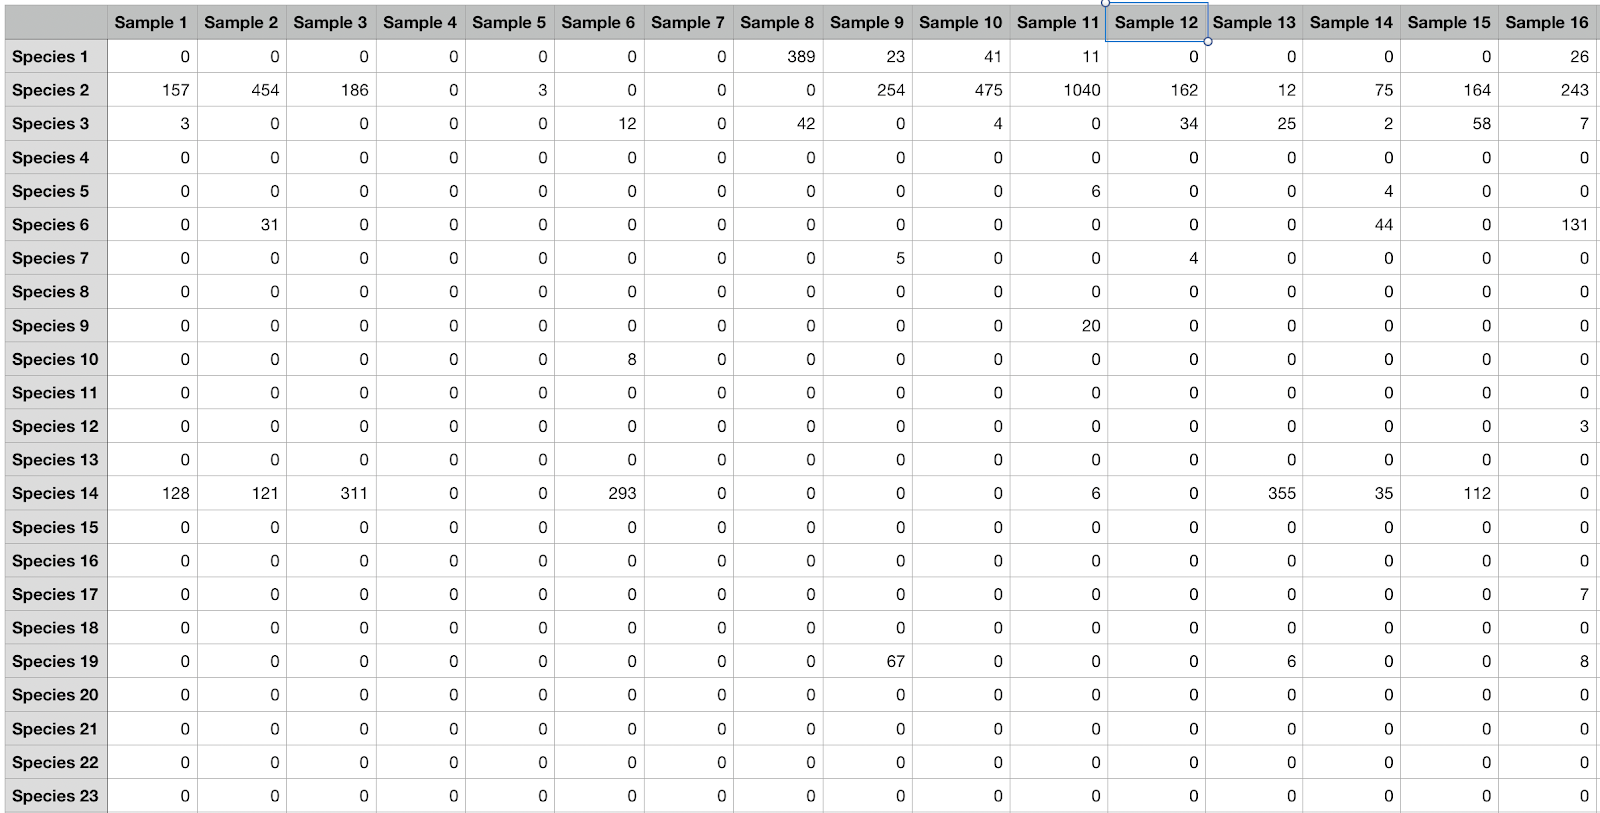
\includegraphics[width=\linewidth]{abundance.png}
  \caption{A Screen Shot of an example of an abundance Table.}
  \label{fig:AbundanceTable}
  \end{center}
\end{figure}

In the data here, a species refers to a specific genetic marker and a sample refers to a physical location where the swab was taken. The values in this table consist of integers, and most of the values are zero. We represent this abundance table as a matrix and call it $A$. We have 
$$A = (a_{ij})_{mn}$$ 
where $m = $ number of species $ = 12311$ and $n = $ number of samples $ = 254$. We also know $a_{ij} \in \N$ and that $59363$ is the maximum value in the matrix. We find that $1.4457\%$ of the values are nonzero. That's about $45,207$ values out of $3,126,994$ values are nonzero. 

To begin to understand what is happening here, we start by creating some histograms and scatter plots. We consider the following analysis on sample sites, referring to each sample as a vector. To start we look at the number of species present at each sample. we say a species is present if it's entry in that column is nonzero. We do this in two manners, we have an abundance histogram which takes into account how many counts of the species were present and the presence histogram which only takes into account whether the species was present or not. Lastly, we look at a presence vs abundance scatter plot to see whether high abundance is correlated with high presence. 


\begin{figure}[H]
\begin{center}
  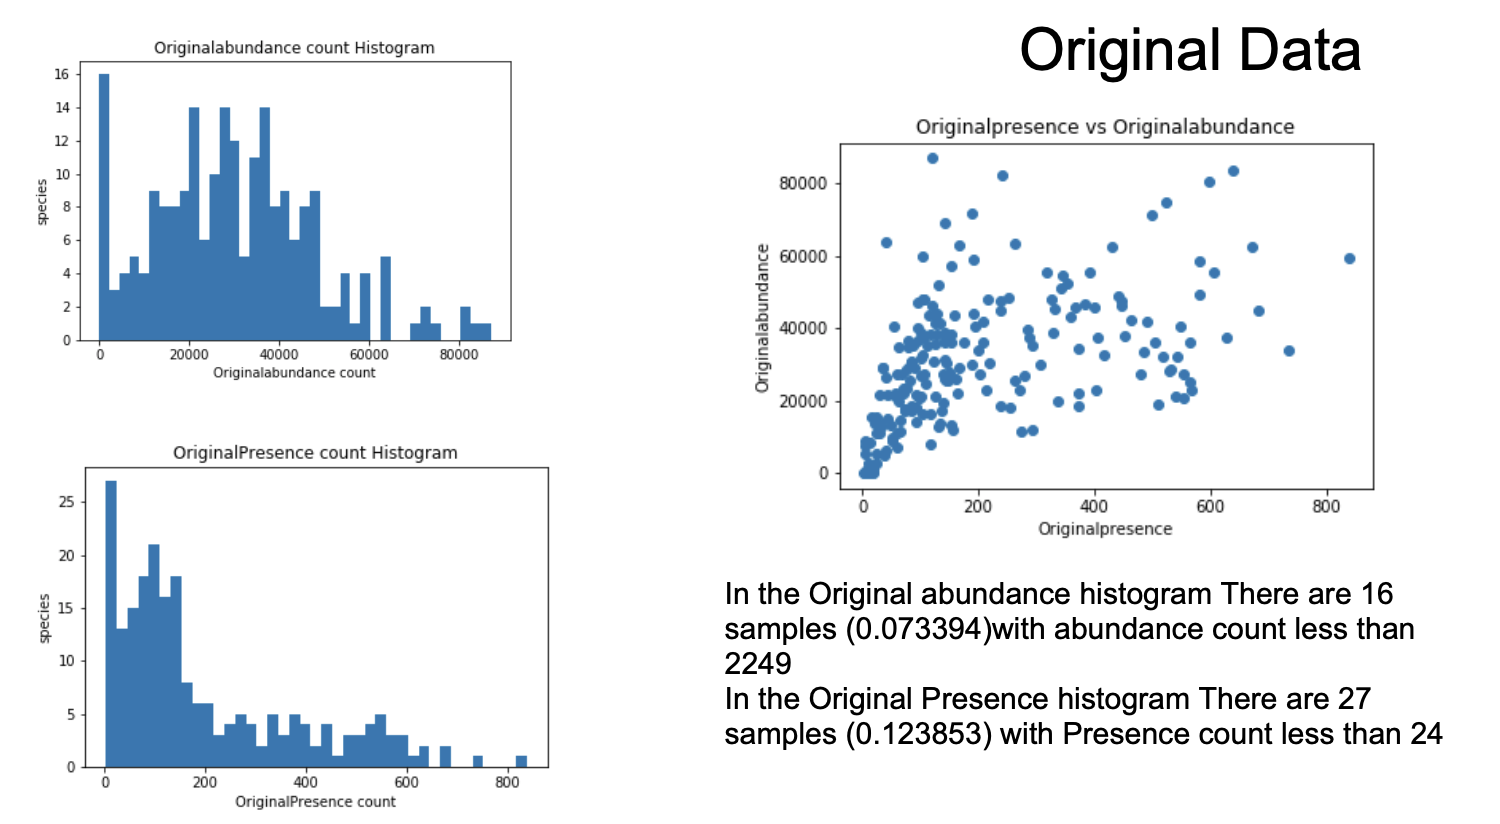
\includegraphics[width=.8\linewidth]{OriginalDataOverview.png}
  \label{fig:OgDataOverview}
  \caption{\textbf{ Error:} The y label axis is wrong. It should say Samples}
  \end{center}
\end{figure}



The abundance histogram shows that a few samples have close to zero abundance, but most samples have a good level of abundance. The presence histogram shows that most samples  have low presence counts. This agrees with the scatter plot that shows that quite a few samples have high abundance but low presence. Given that the data was collected off of everything, this makes sense that things like insect guts would have low presence and low abundance, things like plant leaves would have high abundance and low presence, and things like soil and rocks would have high abundance and high presence as insect guts won't have large varieties or quantities of microbes but rocks will have large varieties and quantities of microbes. 

The next step here is to see if filtering the data had any effect on our understanding of it. This allowed us a better looked at the cluster of data with low presence, so we considered the same set of histograms and scatter plots to see the same pattern at the smaller scale in the histograms, but we see that for sampels with low presence, presence does seem to correlate to abundance. 

\begin{figure}[H]
\begin{center}
  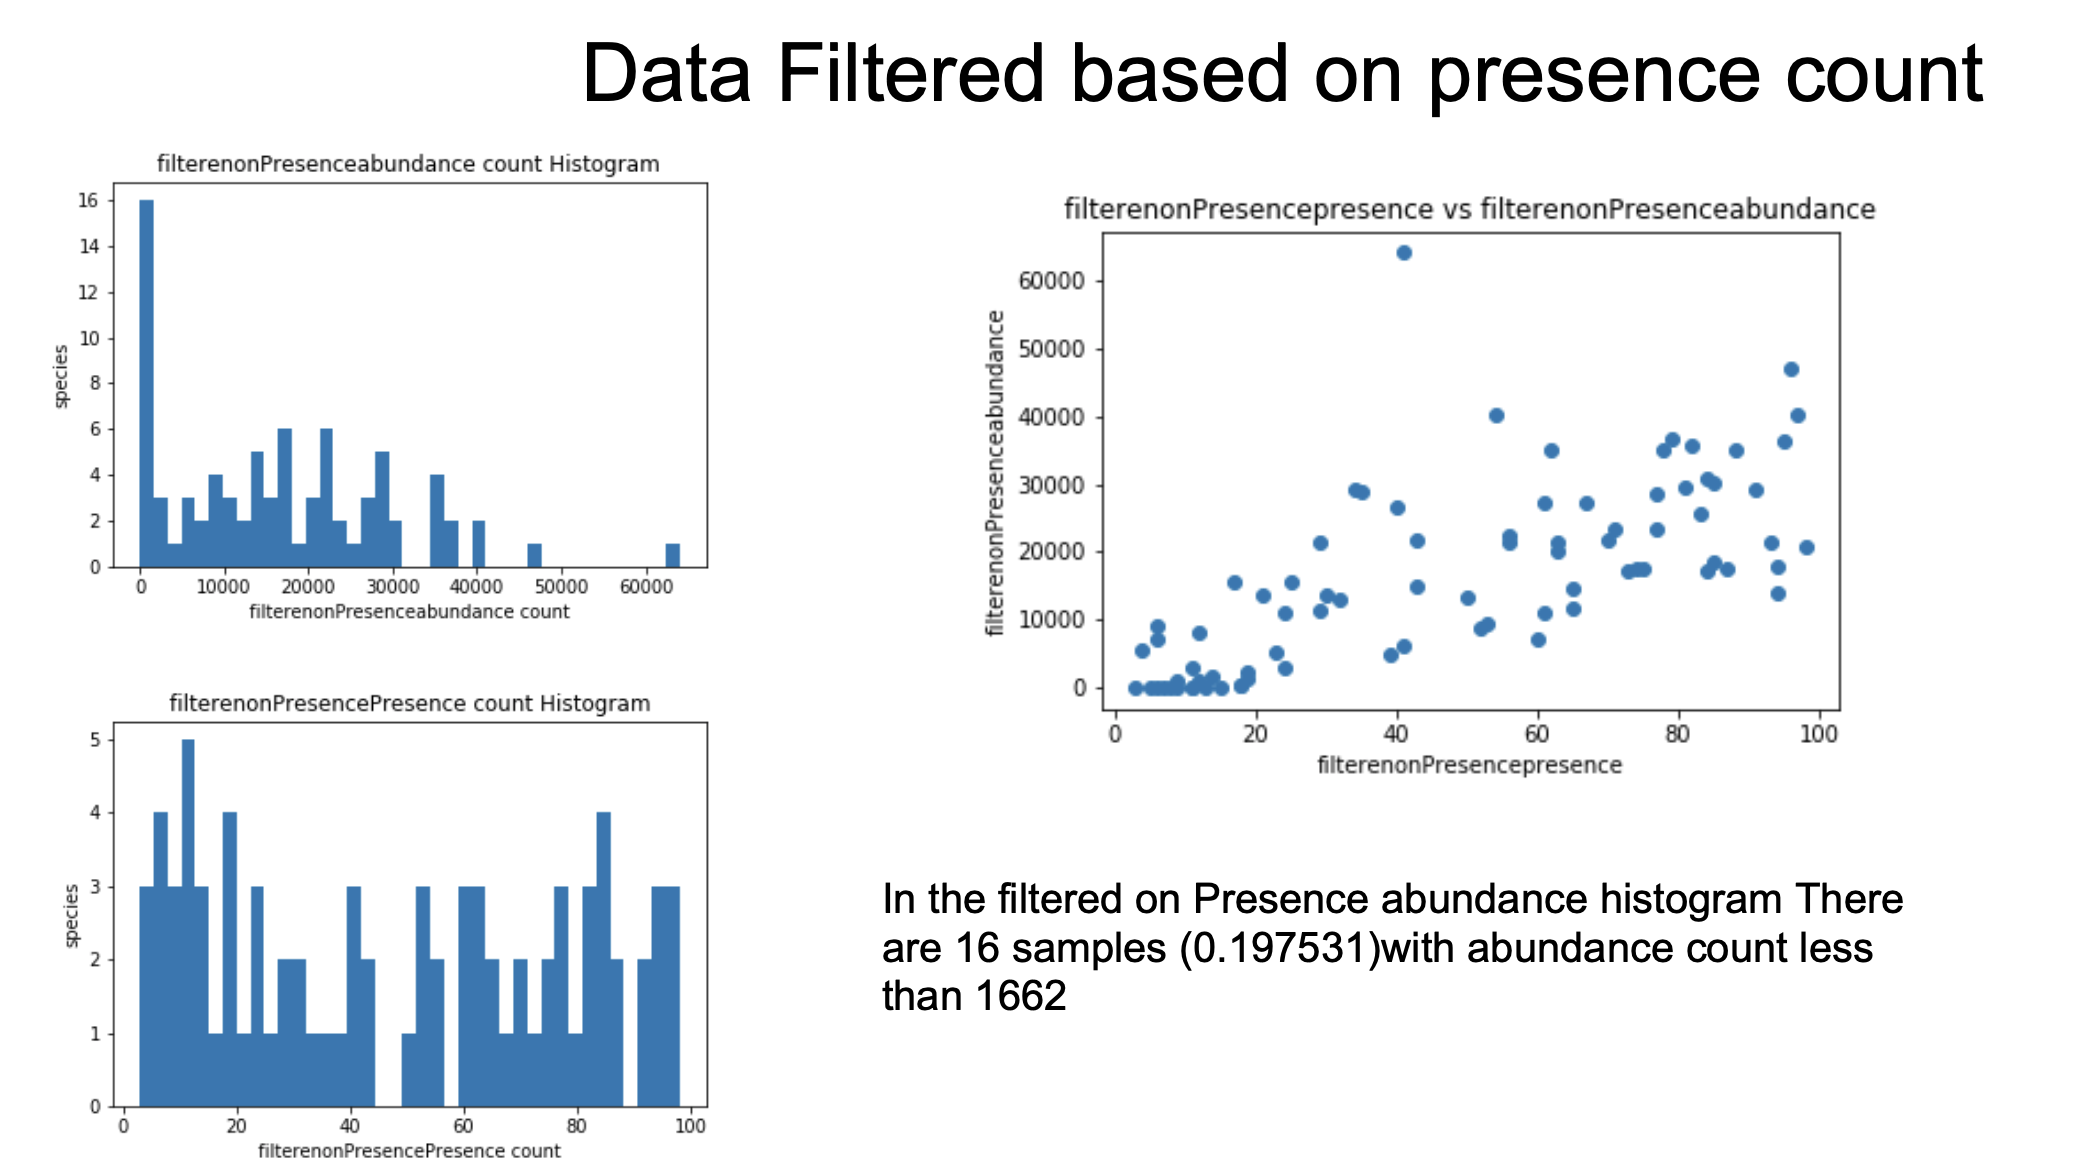
\includegraphics[width=.8\linewidth]{filtdataoverview.png}
  \label{fig:FiltDataOverview}
  \caption{}
  \end{center}
\end{figure}

Next we implemented some qualitative data to see how this changes our understanding of the data. First we start by seeing whether the sample was a terrestrial sample site or a riverine sample site. In each of the following subplots  we will see a black linear regression which gives the relation between presence and abundance for all of the data, the red regression gives the relation for the data with presence below the filtering cutoff which ignores outliers, i.e. samples with really high abundance shown above the green line. 
\begin{figure}[H]
\begin{center}
  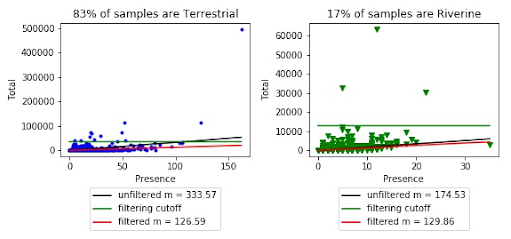
\includegraphics[width=.8\linewidth]{habitat.png}
  \caption{ Scatter plots of sample presence vs abundance split up by land or water sample} 
  \label{fig:habitat}
  \end{center}
\end{figure}

We can see that the majority of the samples collected were collected form a terrestrial site. We can see from the following composite plot that the terrestrial samples have larger presence counts, which means there tends to be a larger variety of microbes on these samples. 
 
 
 
 \begin{figure}[H]
\begin{subfloat}{
  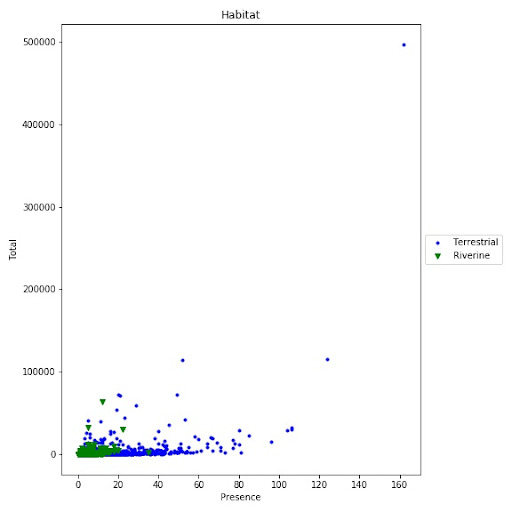
\includegraphics[width=.45\linewidth]{habitatcomp.png}
  \label{fig:habitatcomp}}
\end{subfloat}
\hspace{.1cm}
\begin{subfloat}{
  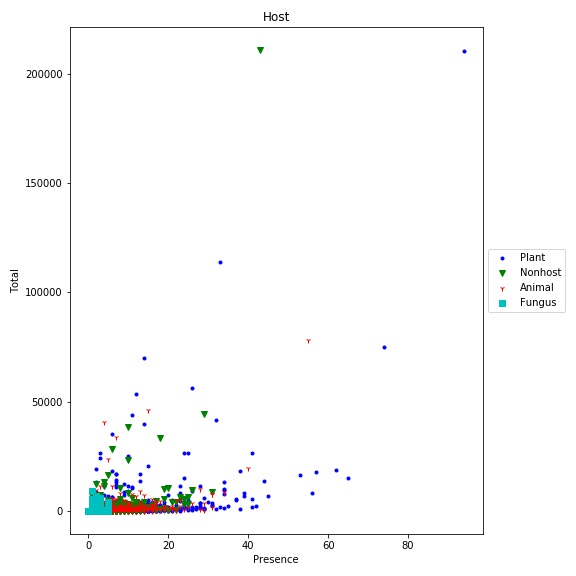
\includegraphics[width=.45\linewidth]{HostPlot.jpg}
  \label{fig:hostcomp}}
  \end{subfloat}
  \caption{ Composite Plot of all samples showing terrestrial and riverine in different colors}
\end{figure}

In the following graph we see the data split up by host. The current data we are working with are all fungal microbes, so when we collected swabs off of mushrooms, we would expect to see low presence of foreign fungal microbes, which we do see. The majority of samples are plant samples. We can also see the data split up by tropic levels, the majority of samples coming from primary producers, which makes sense as the majority of our samples are plants. 

\begin{figure}[H]
\begin{subfloat}{
  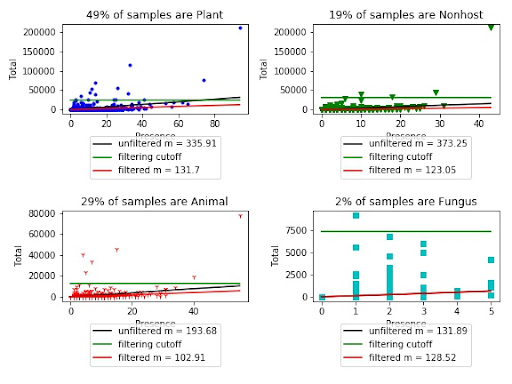
\includegraphics[width=.45\linewidth]{host.png}
  \label{fig:host}}
\end{subfloat}
\hspace{.1cm}
\begin{subfloat}{
  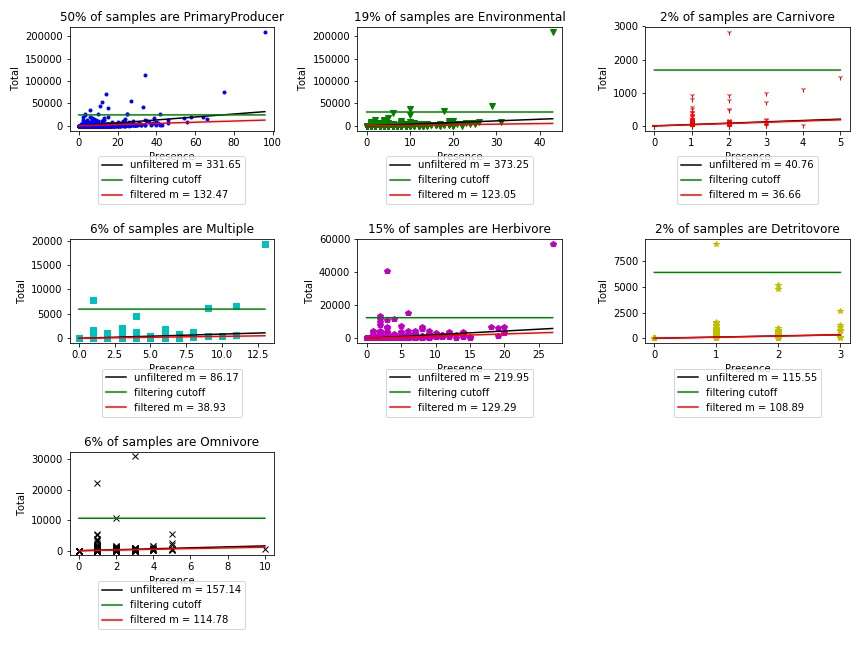
\includegraphics[width=.45\linewidth]{trophic.png}
  \label{fig:trophic}}
  \end{subfloat}
  \caption{}
\end{figure}

In the tropic composite we can see that presence per trophic level does not go much above 40. This means that each sample has about 40 or less various kinds of microbes on it. This can lead us to asking the following question, do the samples have a limit as to how many various kinds of microbes they can carry? Also, we would expect something like soil or rock to carry the largest variety, however we see here that primary producers carry the largest variety of species. 

\begin{figure}[H]
\begin{subfloat}{
  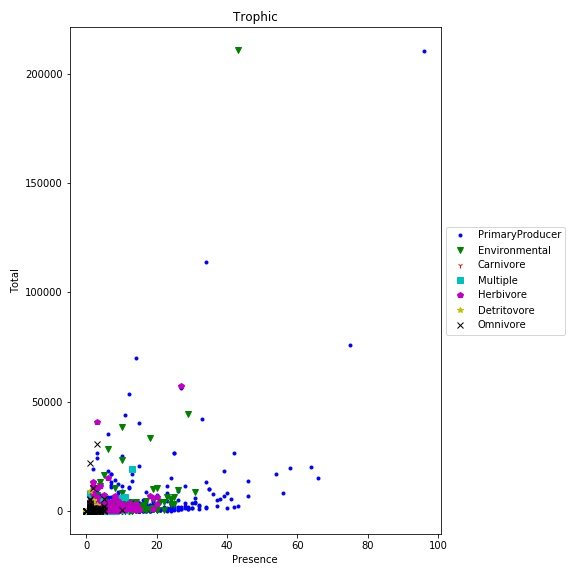
\includegraphics[width=.45\linewidth]{trophiccomp.png}
  \label{fig:trophiccomp}}
\end{subfloat}
\hspace{.1cm}
\begin{subfloat}{
  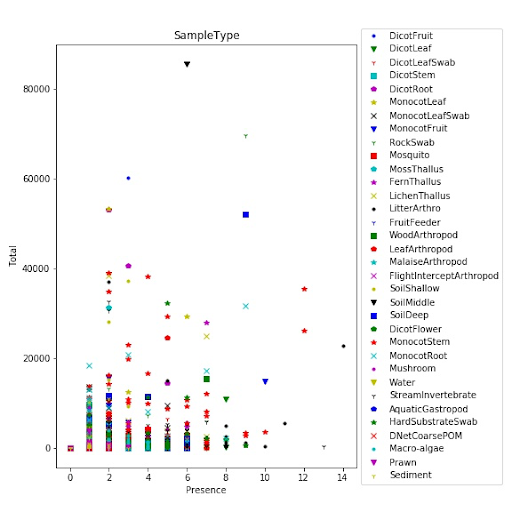
\includegraphics[width=.45\linewidth]{sampleTypecomp.png}
  \label{fig:sampletypecomp}}
  \end{subfloat}
\caption{}
\end{figure}

This last plot splits samples up into sample type, and we see that we have 34 different types of samples, and we see the largest abundance appears in Rock swab, middle soil, and dicot fruit. It would make sense for these to 'hubs' of sorts in a graph display of the data. 
\begin{figure}[H]
\begin{center}

  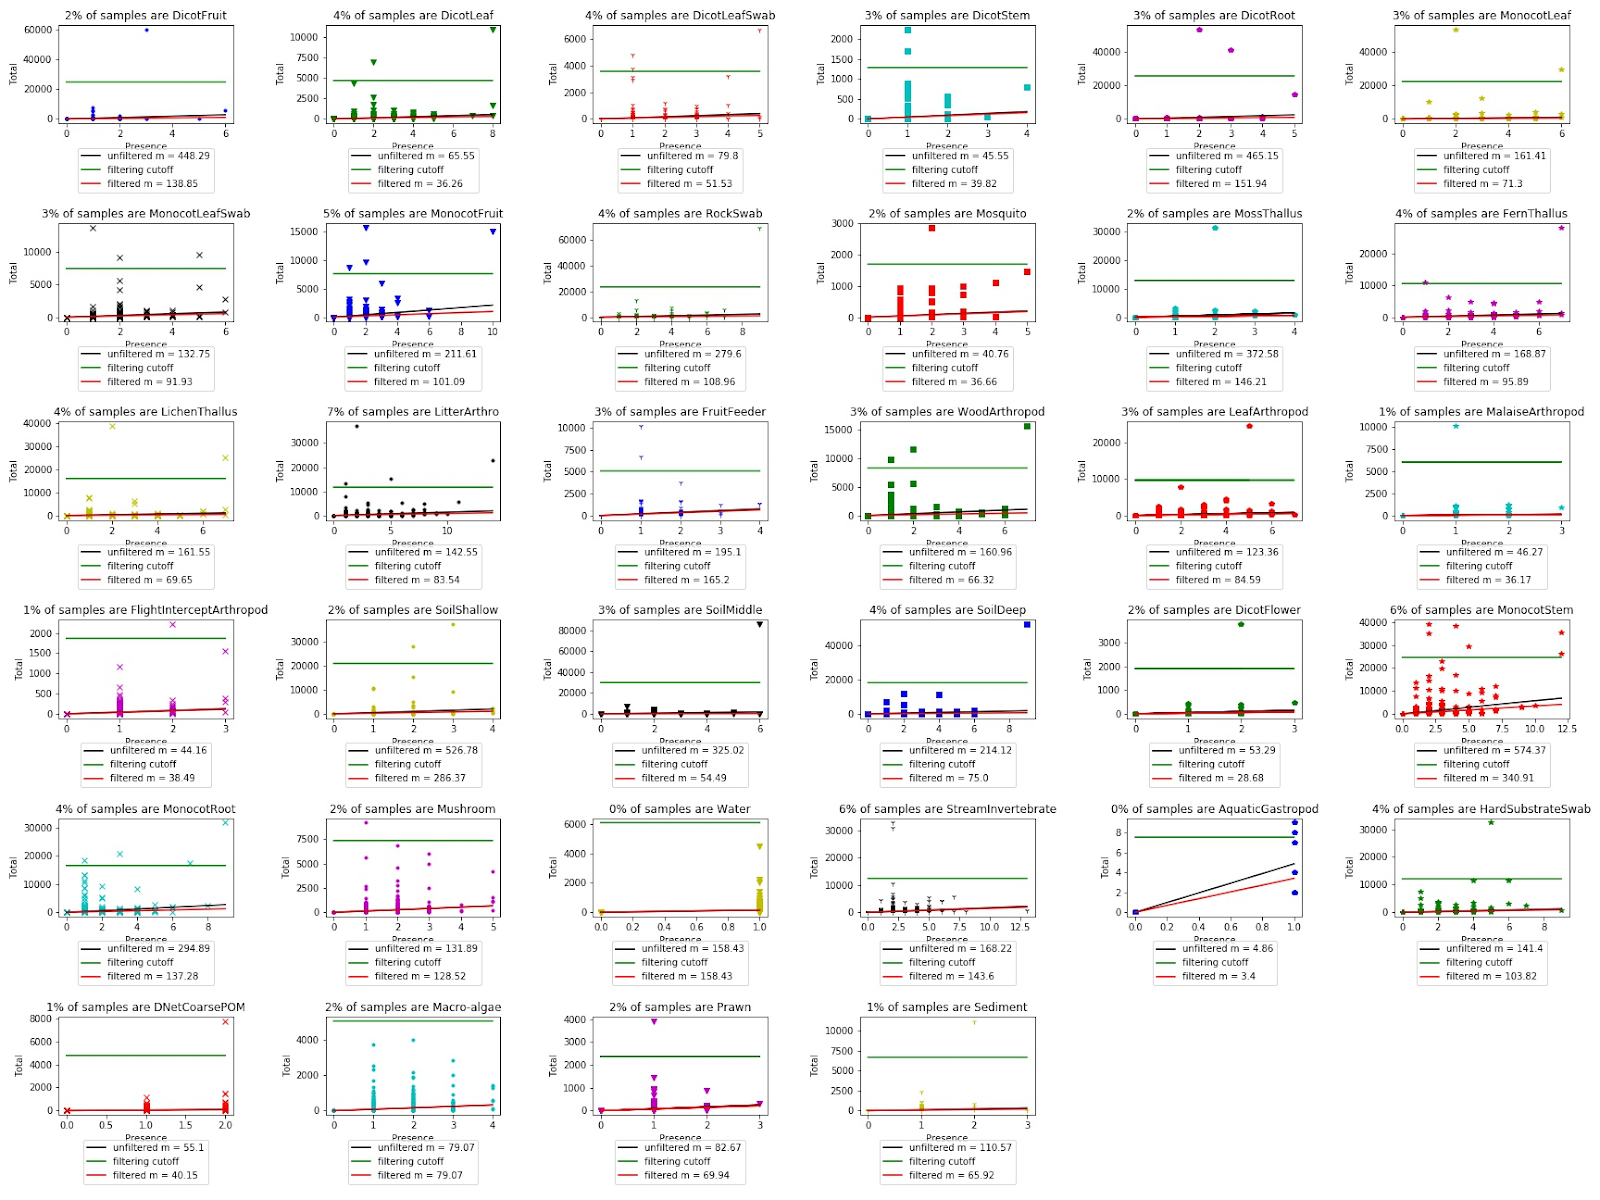
\includegraphics[width=\linewidth]{sampleType.png}
  \caption{Subplots of samples within sample Types}
  \label{fig:samplletype}
  \end{center}

\end{figure}

Now we begin to analyze the data in a more mathematical sense. We will treat the column of our abundance matrix $A$ as vectors in $\R^m = \R^{12311}$. We first start with the abundance table and normalize it. This is done by dividing each entry of the abundance matrix by the column sum. 
$$(\text{Normalized Abundance})_{ij} = \frac{ a_{ij}}{\sum_i a_{ij}}$$
From now on, we refer to the normalized Abundance table as $A$. We can see from this that for a column of our normalized abundance matrix, $\sum_i a_{ij} = 1$. So $a_{ij} \in [0, 1)$ In this setting we see the maximum value that used to be $59363$ is now $0.99889$, and 99$\%$ of the values of $A$ are less than $0.09877$. So there are 452 values of outlier data. 

Now consider some distance metrics. Some standard mathematical metrics employed here are the $\ell_1, \ell_2, \ell_\infty$ metrics, so for two vectors (or columns) $x, y$ we have that these metrics are given by: 
$$ d_1(x,y) = \sum_i |x_i - y_i| \qquad d_2(x,y) = \sqrt{\sum_i|x_i - y_i|^2} \qquad d_\infty(x, y) = \max(|x_i - y_i|)$$
Additionally to these we consider the Bray Curtis dissimilarity. this is not quite a metric as it is not a positive definite function. They Bray-Curtis Dissimilarity for two vectors $x, y$ is given by 
$$d_{BC}(x,y) = 1 - \frac{\sum 2\min(x_i, y_i)}{\sum x_i + \sum y_i}$$


To implement this, we create a new matrix called a distance matrix,  $DM$, which is going to be a symmetric matrix with zeros on the main diagonal. this matrix can be assembled using any of the norms discussed above. This is done for $x_j$ a column vector of the abundance matrix. Since we have about $254$ columns, we have that $DM \in \R^{254 \times 254}$ For the purposes of storage, this matrix is stored as one vector containing the upper triangular entries not including the diagonal entries. 
$$DM_{ij} = d(x_i, x_j)$$
stored for $i = 1, 2, \cdots 254, j = i+1, \cdots 254$. 
Distance Matrix Heat maps are shown for the 1 norm, 2 norm, and Bray-Curtis dissimilarity. 
\begin{figure}[H]
\begin{center}
\begin{subfloat}{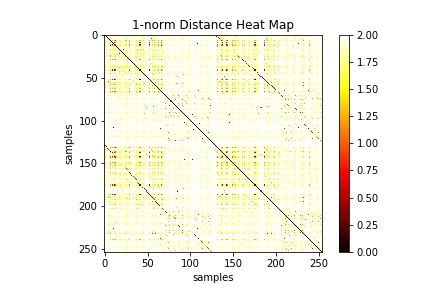
\includegraphics[width=.3\linewidth]{1normHeatmp.jpg}}
\end{subfloat}
\begin{subfloat}{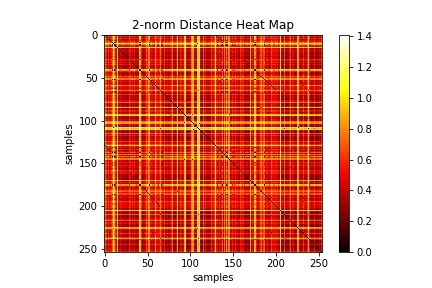
\includegraphics[width=.3\linewidth]{2normHeatmp.jpg}}
\end{subfloat}
\begin{subfloat}{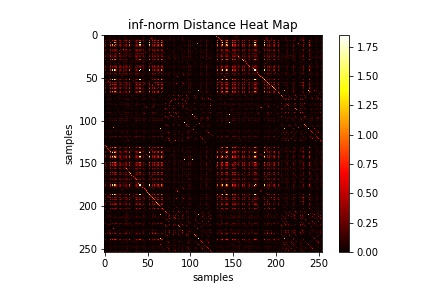
\includegraphics[width=.3\linewidth]{WikiBrayCurtisHeatmp.jpg}}
\end{subfloat}
\caption{ Heat maps of the Distance Matrix. Notice that the Bray-Curtis looks inverted, This is because the dissimilarity is 'inverted' in a sense. \textbf{ Error} The title on the Bray-Curtis matrix is wrong }
\end{center}
\end{figure}

In all of these matrices we can see that the darker the color, the 'closer' the two columns are. Here to say two columns are close is to say that two samples have similar profiles of microbes in presence and abundance. 

We use this distance matrix to generate a weighted graph, and we use the samples as nodes, and the distance between samples as the weights. To understand the weights better, we compile them into one weights vector and look at its distribution. 

\begin{figure}[H]
\begin{center}
\begin{subfloat}{
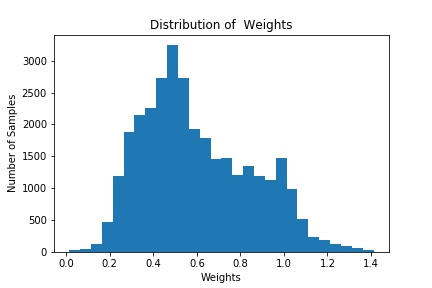
\includegraphics[width = .4\linewidth]{Weights.jpg}}
\end{subfloat}
\begin{subfloat}{
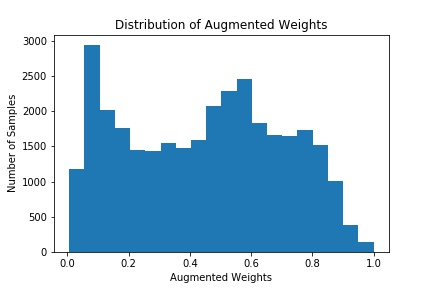
\includegraphics[width = .4\linewidth]{AugWeights.jpg}
}\end{subfloat}
\caption{The weights on the left are skewed, we augment the weights for a better graph distribution, (Right). }
\end{center}
\end{figure}

We can see that the data is skewed, and to better understand our graph, we redistribute the weights to get a normal distribution, or as close to one as possible. To do this, we consider each distance $d(x_i, x_j)$ and we rescale using exponentials. 
$$d(x_i, x_j) \mapsto e^{-\frac{d(x_i, x_j)^2}{\sigma^2}}$$
Using this metric, two vectors that are close will have a distance close to 1, while vectors further apart will be closer to 0. We choose $\sigma$ so the data is as normal as possible, so for our dataset we chose $\sigma$ as the $60.374$ percentile of the data. This gave a skew value of $-6.4\times 10^{-6}$, or in other words, 5 digits of precision to 0. We can see the distribution on the right of Figure 10. We can see how this new augmented weight looks in terms of our heat maps from figure 9 as follows: 

\begin{figure}[H]
\begin{center}
\begin{subfloat}{
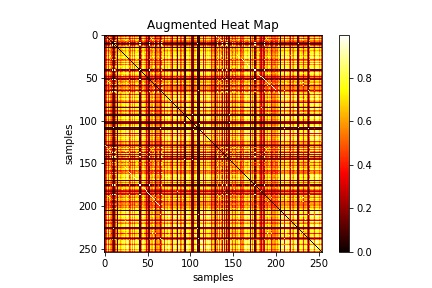
\includegraphics[width = .4\linewidth]{AugmentedHeatMap.jpg}
}\end{subfloat}
\begin{subfloat}{
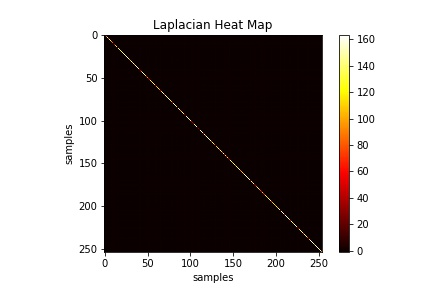
\includegraphics[width = .4\linewidth]{LaplacianHeatMap.jpg}
}\end{subfloat}
\caption{ Visual representation of Connectivity matrix: Heat map of exponentiated distances. Note the diagonal in this matrix is hard coded to be zero when all values on the diagonal should be 1. This allows computation of the laplacian to be more straightforward. On the right is a visual representation of the Laplacian matrix. As the diagonal is the row sum, it makes sense that it is much larger than the off diagonal parts, which are small and negative. }
\end{center}
\end{figure}

We use this new matrix, we'll call it a (weighted) connectivity matrix and we use it to compute the laplacian matrix. To do this we first need to find the degree matrix. The Degree of each node is the sum of the weights of all the nodes that connect to it. This corresponds to the row sum of each row of the connectivity matrix. Note that the diagonal is hard coded to be zero. This vector is put into the form of a diagonal matrix and the graph Laplacian is given by the connectivity matrix $C$ subtracted from the degree matrix $D$. So the laplacian $L$ has the form 
$$L = D - C = \begin{bmatrix} 
\sum_j c_{1, j} && c_{1, 2} && \cdots && c_{1, 254} \\
c_{2,1} && \sum_j c_{2, j} && \cdots && c_{2, 254} \\
\vdots && \vdots && \ddots && \vdots \\
c{_254, 1} && c_{254, 1} && \cdots && \sum_j c_{254, j} 
\end{bmatrix}$$
Where the summations replace the zeros on the diagonal. One thing to note here is that $L*1 = 0$ where $1$ is a vector of ones, and $0$ is the zero vector. This means that $0$ is eigenvalue of the laplacian $L$. We can compute further eigenvalue and eigenvectors fo this matrix. In particular looking at the smallest nonzero eigenvalue, $\lambda_2$ and it's corresponding eigenvector, often called the Fiedler vector in spectral analysis, will allow us to look at clusterings and outliers in our data. When computed we get 
$$\lambda_2 = 13.939538437806185$$ 
and we can see the entries of the eigenvector are represented in Figure 12. 

\begin{figure}[H]
\begin{center}
\begin{subfloat}{
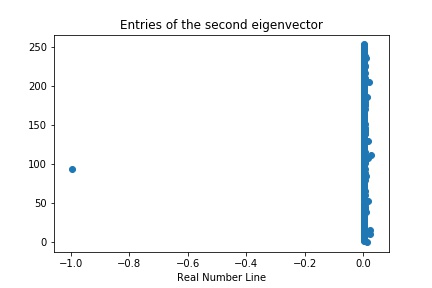
\includegraphics[width = .4\linewidth]{Eigvector.jpg}
}\end{subfloat}
\caption{ Visual representation of the eigenvector that corresponds to $\lambda_2$. The vertical axis corresponds to the entry number, and the horizontal axis represents the value of the entry}
\end{center}
\end{figure}

From spectral analysis we know that for the eigenvector $v$, $\sum_{i = 1}^{254} v_i = 0$, which this does, and positive values and negative values give clusterings of data. What we see in Figure 12 is that one sample is an outlier compared to the rest of them. To understand why we look a little into what this sample is. This corresponds to Sample ID: 100318 and has SampleType LichenThallus, Habitat is Terrestrial, Host is Plant, and its Trophic level is PrimaryProducer. This sample has a maximum value of 0.998886 at Species number 48. If you recall, this was the maximum value of the abundance table, and so it makes sense this would be an outlier. 

We can do the spectral analysis again without this value included. In fact, in our next iteration we will remove outliers based on a threshold value $\epsilon$. In the interactive graph that accompanies this analysis, the threshold is given by $\epsilon  \times 10$ We construct a new adjacency matrix by replacing small values in the connectivity matrix with zero. If a sample is an outlier, then it's distance from all other samples will be far away. In the connectivity matrix, samples that are far away are represented with a distance close to zero. By setting this value to zero, we are removing it from our calculations of the degree of the sample, and from our connectivity matrix. We say a distance is close to zero if it is below the threshold. Here we can see the adjacency Matrix for $\epsilon = .2$ and $\epsilon = .8$. 

\begin{figure}[H]
\begin{center}
\begin{subfloat}{
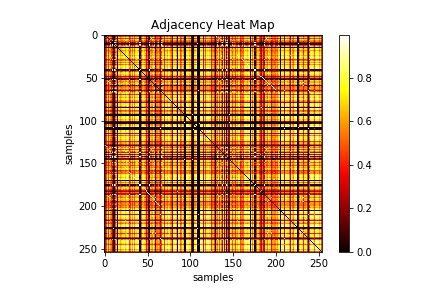
\includegraphics[width = .4\linewidth]{AdjacencyHeatMap.jpg}
}\end{subfloat}
\begin{subfloat}{
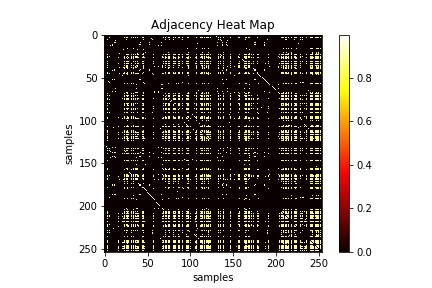
\includegraphics[width = .4\linewidth]{AdjacencyHeatMap8.jpg}
}\end{subfloat}
\caption{Left: $\epsilon = .2$; Right: $\epsilon = .8$}
\end{center}
\end{figure}

We can see in these images that for $\epsilon = .2$ we have close to a complete graph with some sample connections removed for samples around 100. In the $\epsilon = .8$ case we have many connections removed and we're looking at structures that are very close knit and hidden by outside surrounding samples that distantly connect. 

Using these new adjacency matrices, we can calculate the corresponding degree matrices and laplacians using the same method as above. We continue with their eigenvalues and eigenvectors as follows: 

\begin{figure}[H]
\begin{center}
\begin{subfloat}{
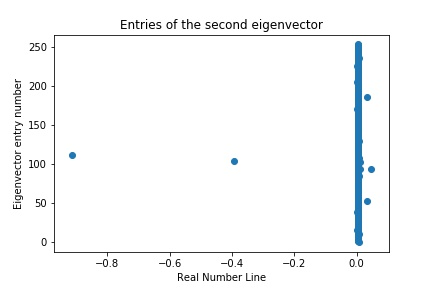
\includegraphics[width = .3\linewidth]{Eigvector2.jpg}
}\end{subfloat}
\begin{subfloat}{
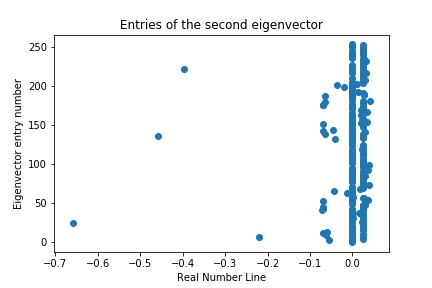
\includegraphics[width = .3\linewidth]{Eigvector8.jpg}
}\end{subfloat}
\begin{subfloat}{
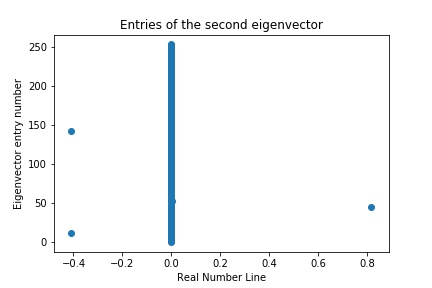
\includegraphics[width = .3\linewidth]{EigvectorEmpty.jpg}
}\end{subfloat}
\caption{Left: $\epsilon = .2$; Center $\epsilon = .8$; Right: $\epsilon = .99$}
\end{center}
\end{figure}

We can see from Figure 14 that when we set our threshold to .2, we still include enough outlier data in our adjacency matrix so that we do not get a good clustering of data. When we increase our threshold to .8, we have gotten rid of most of the outliers and we can see two clear groups of data here. However if we keep increasing the threshold, we remove so much of the data that we're only left with three points that haven't been set to zero. 

\end{document}